\documentclass[10pt,final,a4paper]{article}
\usepackage[left=3cm,right=3cm,top=2cm,bottom=2cm]{geometry}
\usepackage[utf8]{inputenc}
\usepackage{amsmath}
\usepackage{amsfonts}
\usepackage{amssymb}
\usepackage{subcaption}
\usepackage{amsthm}
\usepackage{mdframed}
\usepackage{graphicx}
\usepackage{listings}
\usepackage[square,sort,comma,numbers]{natbib}
\usepackage[dvipsnames]{xcolor}
\usepackage[]{algorithm2e}
\usepackage{bm}
\usepackage{soul}
\soulregister\cite{7}
\makeatletter
\renewcommand{\@algocf@capt@plain}{above}% formerly {bottom}
\makeatother
\newtheorem{theorem}{Theorem}
\newtheorem*{proof*}{Proof}
\newtheorem{lemma}{Lemma}
\usepackage{hyperref}
\newtheorem{assumption}{Assumption}
\newtheorem*{assumptionbis}{Assumption 2-bis}
\newtheorem{definition}{Definition}
\newtheorem{remark}{Remark}
\newtheorem{corollary}{Corollary}
\newcommand{\R}{\mathbb{R}}
\newcommand{\E}{\mathbb{E}}
\newcommand{\V}{\mathbb{V}ar}
\newcommand{\x}{\widehat{x}}
\newcommand{\dd}{\mathrm{d}}
\newcommand\numberthis{\addtocounter{equation}{1}\tag{\theequation}}
\newcommand{\uu}{u^*}
\newcommand{\uuh}{u^{h*}}
\newcommand{\uhu}{\widehat{u}^*}
\usepackage{enumitem}

\setlist[itemize,3]{label=$\diamond$}

\usepackage{calrsfs}
\DeclareMathAlphabet{\pazocal}{OMS}{zplm}{m}{n}
\newcommand{\La}{\mathcal{L}}
\newcommand{\Lb}{\pazocal{L}}


% editing
\newcommand{\FabioAdd}[1]{{\color{magenta} #1}}
\newcommand{\MMAdd}[1]{{\color{teal} #1}}
\newcommand{\FabioCorr}[2]{{\color{red}\st{#1}} {\color{red} #2}}
\newcommand{\FabioMP}[1]{{\color{red} *} \marginpar{\footnotesize \color{red}*Fabio: #1}}
\newcommand{\MattMP}[1]{{\color{blue} *} \marginpar{\footnotesize \color{blue}*Matthieu: #1}}
\newcommand{\SebQ}[1]{{\color{blue}\textbf{Seb:} #1}} %question in text
\newcommand{\SebMP}[1]{\textcolor{blue}{*} \marginpar{ {\begin{flushleft} \scriptsize \textcolor{blue}{* #1} \end{flushleft} } }} % note as a margin par
\newcommand{\SebNew}[1]{{\color{blue} #1}}

% math commands
\def\KL{{Karhunen-L\`{o}eve }}
\DeclareMathOperator*{\argmin}{arg\,min}
\DeclareMathOperator*{\dive}{div}
\DeclareMathOperator*{\essinf}{essinf}

\begin{document}
%\maketitle
% define title information
\title{EE-559: Mini-project II}
\author{Pegolotti Luca - Martin Matthieu \footnote{As agreed with Dr. F. Fleuret, L. Pegolotti has collaborated with group 78 for Project 1 and with group 79, with M. Martin, for Project 2. C. Bigoni and N. Ripamonti have worked together on both projects.}}

\date{\today}
\maketitle


\section{Objective}

The objective of this project is to design a mini “deep learning framework” using only tensor operations in Pytorch and the standard Numpy library, in particular without using autograd or the neural-network modules. 

\section{Code structure}
\begin{figure}
\centering
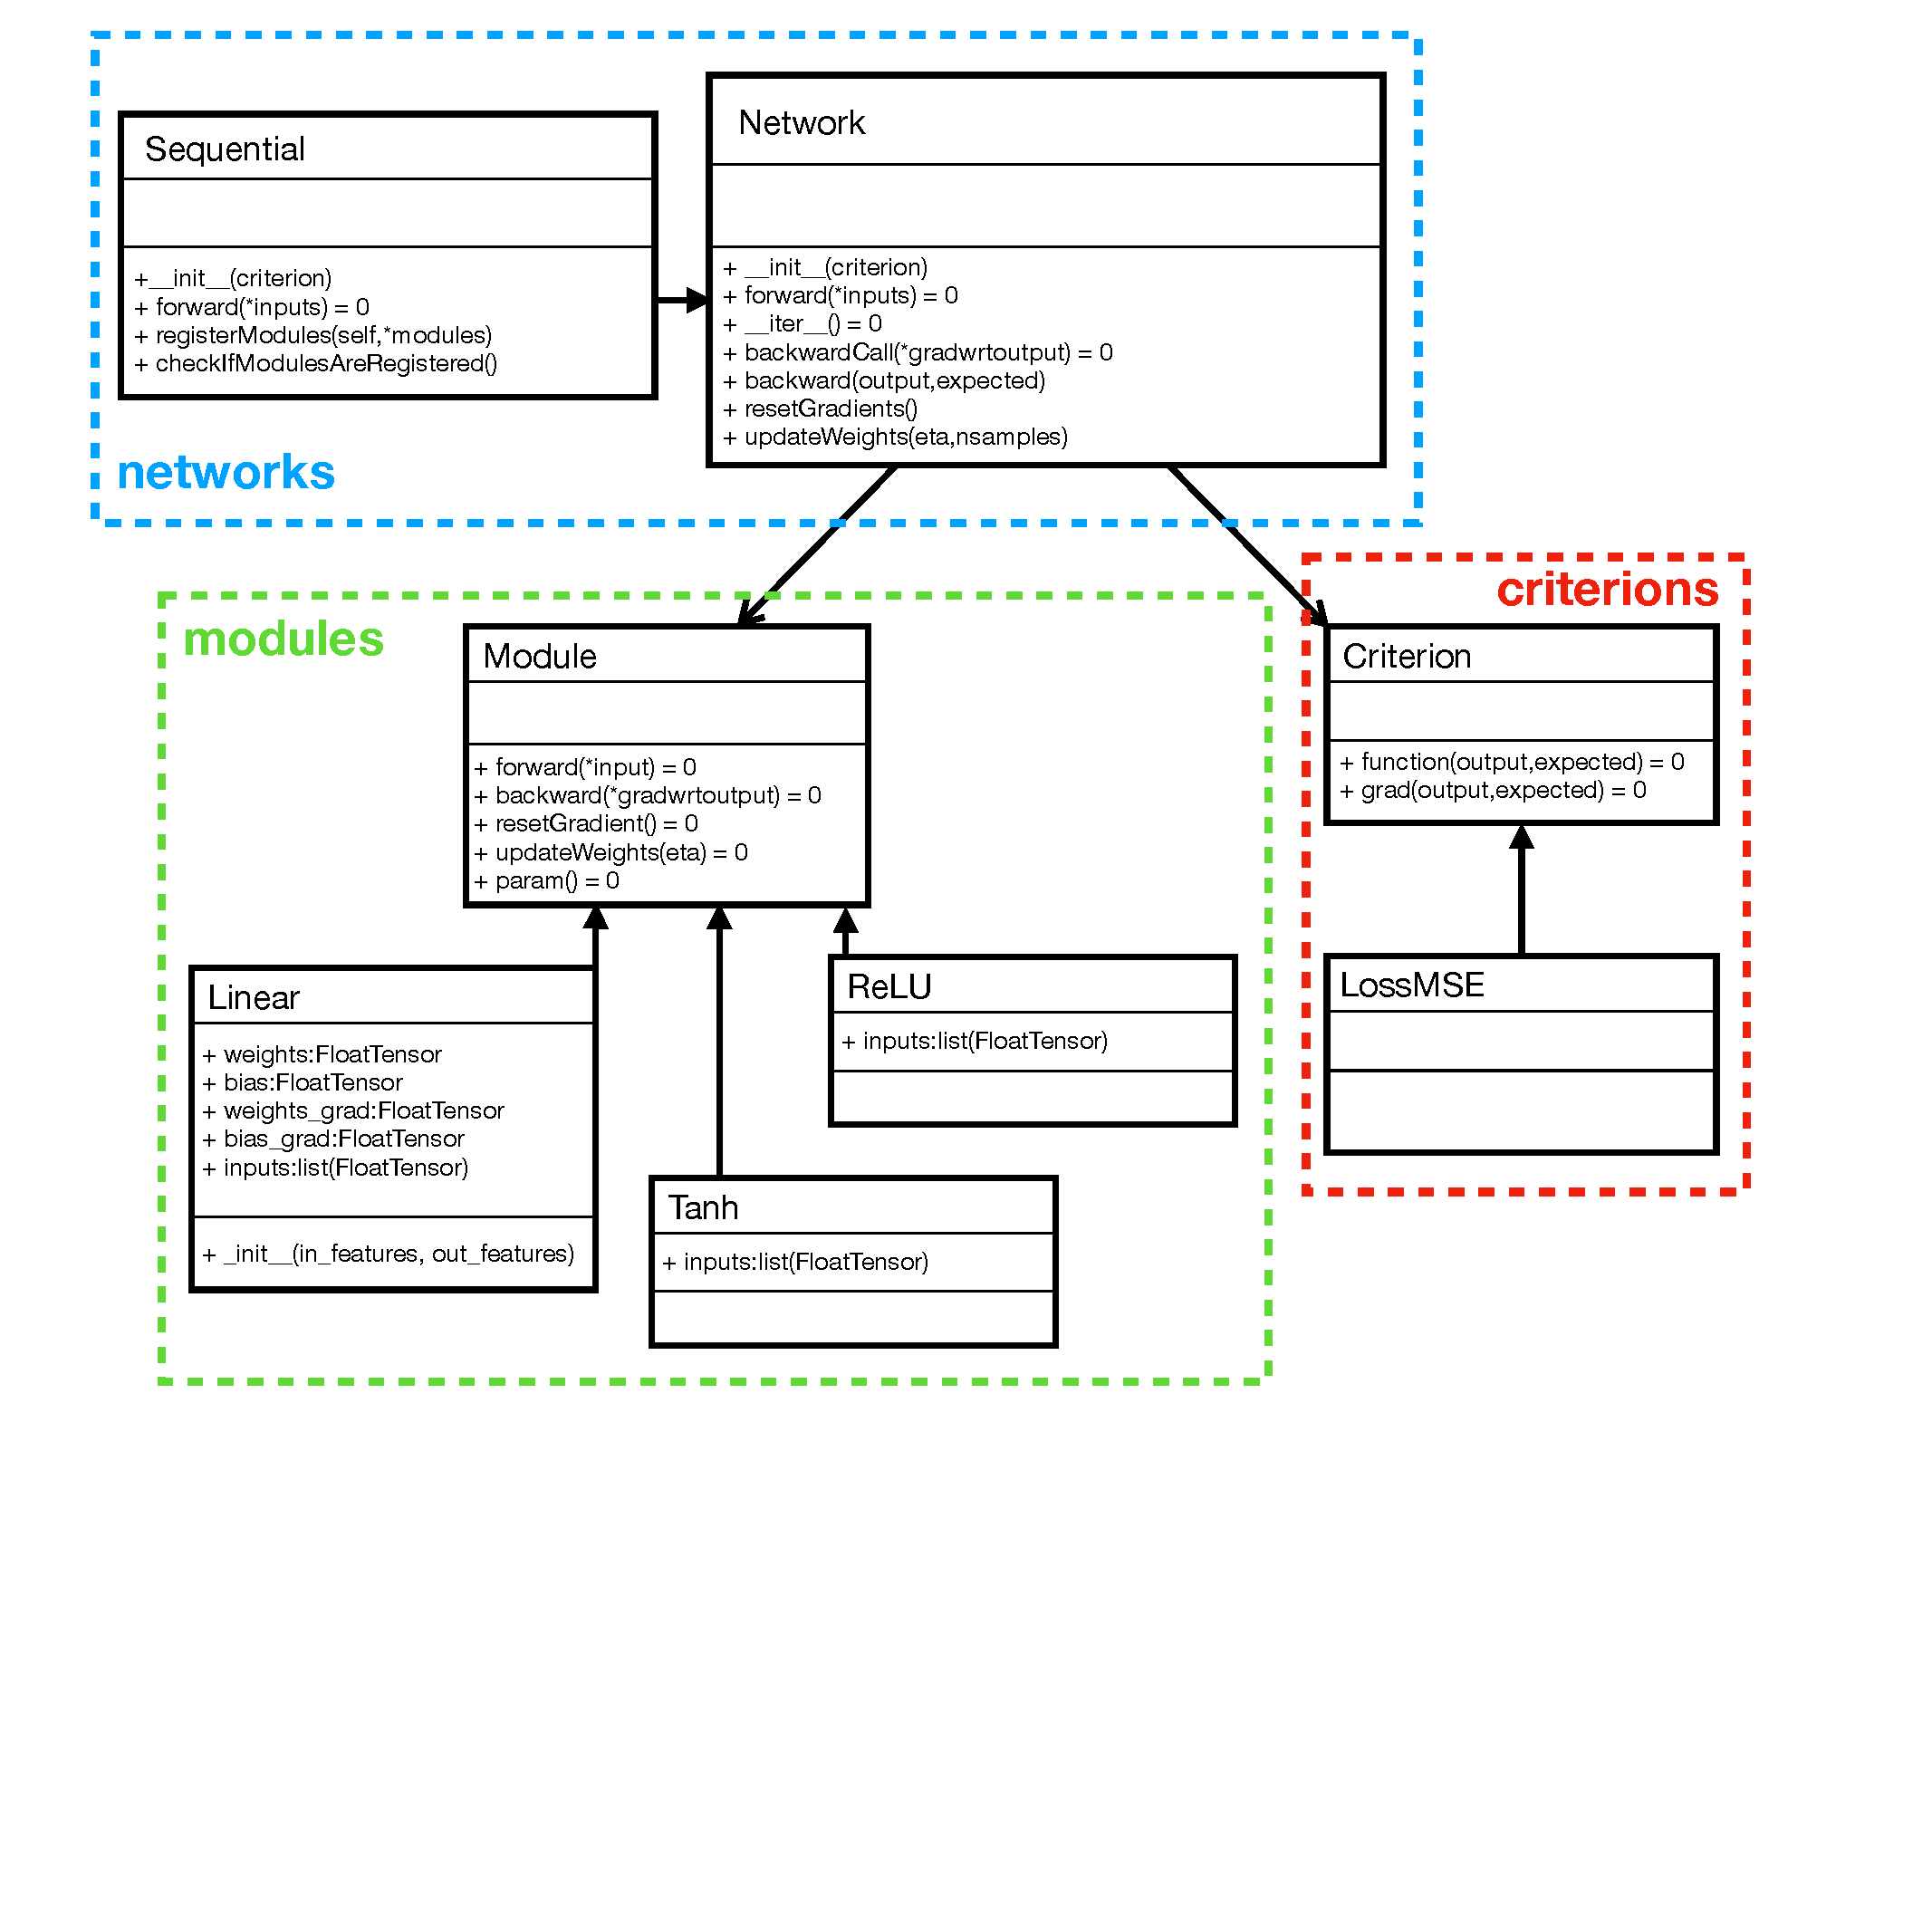
\includegraphics[scale=0.42, clip=true, trim=45 270 0 10]{diagram.pdf}
\caption{Class diagram of the framework. We indicate with the notation ``$=0$'' the methods that need to be implemented by the derived classes, even though such methods are not actually abstract in a strict sense.}
\label{fig:diagram}
\end{figure}
The framework is composed by three modules: \verb|modules|, \verb|criterions| and \verb|networks|, located in the framework/ folder in the root of the project. The classes implemented in each module interact as shown in Figure~\ref{fig:diagram}. A set of tests on these classes is implemented in the framework/testsuite.py script. The code has been tested with Python 3.6.5 and Pytorch version 0.4.0.
\subsection{Modules}
Modules implement some of the typical building blocks of a neural network. Each of these building blocks derives from the class \verb|Module| (see Figure~\ref{fig:diagram}), the basic structure of which (except for the methods \verb|resetGradient| and \verb|updateParameters|) was suggested in the description of the project. The methods \verb|forward| and \verb|backward| implement a forward and backward pass respectively. The method \verb|resetGradient| resets all the gradient tensors (if any) to zero, whereas the method \verb|updateWeights| updates the weights (if any) of the module according to the learning rate \verb|eta|.

All the modules deriving from \verb|Module| posses a variable \verb|input| taking the value of the input which was provided during the latest call to the \verb|forward| method: this is necessary to compute  the \verb|backward| call.
The classes which derive from \verb|Module| are:
\begin{itemize}
\item \verb|Linear|: given an input tensor $x \in \mathbb{R}^{n_\text{s} \times n_\text{in}}$, the output $y \in \mathbb{R}^{n_\text{s} \times n_\text{out}}$ of this module is given by $y_{ij} = \sum_{k} x_{ik} A_{jk} + b_{j}$, where $A \in \mathbb{R}^{n_\text{out} \times n_\text{in}}$ is the weight matrix, $b \in \mathbb{R}^{n_\text{out}}$ is the bias, and $n_\text{in}$, $n_\text{out}$ and $n_\text{s}$ are the number of input/output features and samples respectively. This module has the attributes \verb|weight| and \verb|bias|, which store the values of $A$ and $b$ respectively, and \verb|weight_grad| and \verb|bias_grad| which store the respective gradients. In the backward pass, the module accepts as input the gradient of the loss function computed with respect to its output (this is computed by the nodes that immediately follows in the network) which we denote by $\partial \Lb/\partial y$. Then, the gradients of the loss with respect to the weights and bias are found as $\partial \Lb/\partial A = (\partial \Lb/\partial y)^T x$ and $\partial \Lb/ \partial b = \sum_{j} (\partial \Lb/\partial y)_j$, where $\partial \Lb/\partial A \in \mathbb{R}^{n_\text{out} \times n_\text{in}}$, $\partial \Lb/\partial y \in \mathbb{R}^{n_\text{s} \times n_\text{out}}$, $\partial \Lb/ \partial b \in  \mathbb{R}^{n_\text{out}}$, and  $(\partial \Lb/\partial y)_j$ denotes the $j^{\text{th}}$ row of $\partial \Lb/\partial y$. The gradient of the loss with respect to the input of the module, which is to be passed to the previous node in the network, is found as $\partial \Lb / \partial x = \partial \Lb/\partial y A$.
\item \verb|ActivationFunction|: interface which provides a default implementation to the methods in  \verb|Module| that operate on or require internal weights or gradients. The backward pass of a generic activation function $\sigma$ takes as argument the gradient of the loss function with respect to the output of the module, $\partial \Lb/\partial y$, and passes to the previous node the derivative of the loss function with respect to its input $x$, which is computed as $\partial \Lb/\partial x = \partial \Lb/\partial y \odot \sigma'(x)$. Classes which inherit from this template are:
\begin{itemize}[label={$\diamond$}]
\item \verb|ReLU|:  this module applies the ReLU function to any given input tensor, namely, given $x \in \mathbb{R}^{n \times m}$, the output tensor $y \in \mathbb{R}^{n \times m}$ is defined by $y_{ij} = \text{ReLU}(x_{ij}) = \text{max}\{0, x_{ij}\}$.
\item \verb|Tanh|: this module applies the tanh function to each component of the input tensor $x \in \mathbb{R}^{n \times m}$, i.e. the output tensor  $y \in \mathbb{R}^{n \times m}$ is defined by $y_{ij} = \text{tanh}(x_{ij})$, where
\begin{equation*}
\text{tanh}(x) = \dfrac{e^x - e^{-x}}{e^{x} + e^{-x}}.
\end{equation*}
\item \verb|Sigmoid|: this module applies the sigmoid function to the given input tensor. If $x \in \mathbb{R}^{n \times m}$ is the input tensor, then $y_{ij} = \text{sigmoid}(x_{ij})$ and $y \in \mathbb{R}^{n \times m}$. The sigmoid functions is defined as
\begin{equation*}
\text{sigmoid}(x) = \dfrac{e^x}{e^x + 1}.
\end{equation*}
\end{itemize}
\end{itemize}
\subsection{Criterions}
The \verb|criterions| module contains the implementation of the loss functions. These share the interface given by the following base class \verb|Loss| (see Figure~\ref{fig:diagram}). The method \verb|function| computes the loss function of the \verb|output| of a forward pass of a network with respect to the target (\verb|expected|), and the \verb|grad| method computes the gradient of the loss corresponding to the same parameters.

The available criterions are:
\begin{itemize}
\item \verb|LossMSE|: Mean Square Error loss function. If $x \in \mathbb{R}^{n \times m}$ is the output of the forward pass and $y \in \mathbb{R}^{n \times m}$ is the expected output, the loss function is computed as
\begin{equation*}
\text{MSE}(x,y) = \dfrac{1}{N} \sum_{i,j} (x_{ij} - y_{ij})^2,
\end{equation*} 
where $N$ is the total number of entries of the tensors $x$ and $y$.
\item \verb|LossCrossEntropy|: to be implemented?
\end{itemize}

\subsection{Networks}
The \verb|criterions| module provides generic structures for the implementation of neural networks. The base class is the \verb|Network| class (see Figure~\ref{fig:diagram}). Each derived class must be iterable (namely, it must provide the abstract method \verb|__iter__|) and must implement the \verb|forward| and the \verb|backward| methods, which depend on the topology of the underlying graph.

The available networks are:
\begin{itemize}
\item \verb|Sequential|: template for neural networks: it provides a blueprint for derived classes implementing fully connected neural networks. Each graph must include a unique ``source'' (a node with only one input), a unique ``sink'' (a node with only one input) and nodes with exactly one input and one output. Each node is in fact an object derived from the \verb|Module| class and must be defined as an attribute of a derived class in the constructor. Importantly, at the end of the constructor these objects must be registered via the method \verb|registerModules(self,*modules)|, where the \verb|*modules| must contain the modules in the order they appear in the network itself. Internally, the \verb|registerModules| method builds a list of the modules, which  provides a way to iterate over the elements composing the \verb|Sequential| network. The forward and backward passes are executed in a straightforward manner by calling the \verb|forward| and \verb|backward| method of all the modules of the graph sequentially and propagating the result to the next or the previous node (the gradient to be injected in the last node of the network is the gradient of the loss functions with respect to the output of the forward pass).
\end{itemize}
\section{Test case}
The structure of the test code, implementing a network with two input units, two output units, three hidden layers of 25 units is:
\begin{itemize}
\item Generate 1000 training sample, and 1000 testing points\\
\item Normalize them with a zero mean and unit std\\
\item Built a three hidden layer with linear neural network, and ReLU after each linear module "SimpleNet"\\
\item Train the neural network using the 1000 training sample, for 1000 epochs and a constant learning rate $=1e-2$.
\item Plot the training error and the testing error while training the network, and verify these results with the framework PyTorch.
\end{itemize}

The parameters of the sample length is hidden in the $mean$ function, and we had to modify the eta in the final code: $eta=eta/nsample$.
\begin{verbatim}
class LossMSE(object):
    def function(self,output,expected):
        return torch.mean(torch.pow(expected - output,2))

    def grad(self,output,expected):
        return -2 * (expected - output)
\end{verbatim}

The sequential class work as follow:
\begin{verbatim}
class Sequential(Module):
    def __init__(self,criterion):

    def registerModules(self,*modules):

    def checkIfModulesAreRegistered(self):

    def resetGradient(self):

    def updateParameters(self,eta,nsamples):

    def backward(self,*gradwrtoutput):

    def backwardPass(self, output, expected):

\end{verbatim}
where the $registerModules$ needs to be called when we define a new network, in order to store the modules in a list. We will use the list ordered when we will call the methods $forward$, $backward$, and $update_Parameters$

\section{Conclusion}
We have presented a simplified framework for neural networks that allows to easily concatenate building blocks (modules) sequentially. The simple numerical test we implemented shows that the stochastic gradient descent converges and that the errors we obtain on train and test datasets are small and comparable to the ones found when solving the same problem with Pytorch. 

With the goal of imitating the user-friendly interface of Pytorch, we came up with a solution to generate customized neural networks that require the definition of the modules inside the constructor of the \verb|Network| subclass and the implementation of a \verb|forward| method. We believe that the structure of the code is well-suited to be extended to other modules (e.g. convolutional layers, pooling \ldots) or to account for more complicated networks. However, our solution consists in internally storing the modules into a list, and therefore does not account for situations in which some nodes require multiple inputs/outputs. The major obstacle to the generalization of the approach to more complicated networks lies in the auto-generation of the underlying graph. A possible way to overcome this issue, in our opinion, could consist in introducing a wrapper for the tensor passed along the graph (similarly to what is done in Pytorch, with the Variable class) in which also the information of the latest visited node is stored. This could allow to build the graph ``on the fly" during the forward pass and to propagate the information backward in the back propagation algorithm.

\end{document}
\grid
